\chapter*{Preface}
\addcontentsline{toc}{chapter}{Preface}
Theses at the faculty of mathematics and physics usually fit into one of three categories:
\begin{enumerate}
\item Theoretical thesis
\item Experimental thesis
\item Implementation thesis
\end{enumerate}
My thesis does not fit entirely into only one category and it does not try to. The project consists of several similarly important parts which are:
\begin{itemize}
\item Design of the algorithm for generating a special binary matrix
\item Making it run fast on inputs which are usual for researchers
\item Implementing the algorithm to provide practical tool
\end{itemize}
None of these points would make sense alone but together the thesis may become very useful for scientists as it is a common practice to test hypothesis on random data.
\chapter*{Introduction}
The area of pattern avoidance is heavily studied for permutations and it also becomes studied more for its generalization - binary matrices.

We denote by $M\in\{0,1\}^{n\times m}$ a binary matrix of size $n$ by $m$, calling $n$ the number of rows of $M$ - the height of the matrix $M$ and $m$ the number of columns - its width. A line of a matrix is one of its rows or columns and for matrix $M$, we denote $L(M)$ the ordered set of all lines of $M$. Its order is given by the natural indexing of rows and columns.

We say a binary matrix $M$ contains a binary matrix $P$, which we call a ``pattern'', as a submatrix, if there is a mapping $f:L(P)\rightarrow L(M)$, such that
\begin{itemize}
\item $l\in L(P)$ is a row of $P$ iff $f(l)\in L(M)$ is a row of $M$
\item $\forall l,l'\in L(P):$ $l<l'\Rightarrow f(l)<f(l')$ (preserves the order)
\item $\forall l,l'\in L(P):$ if lines $l$ and $l'$ intersect and there is a one-entry at the intersection, then there is a one-entry at the intersection of $f(l)$ and $f(l')$.
\end{itemize}
otherwise, it avoids the pattern $P$.

\centerline{\mbox{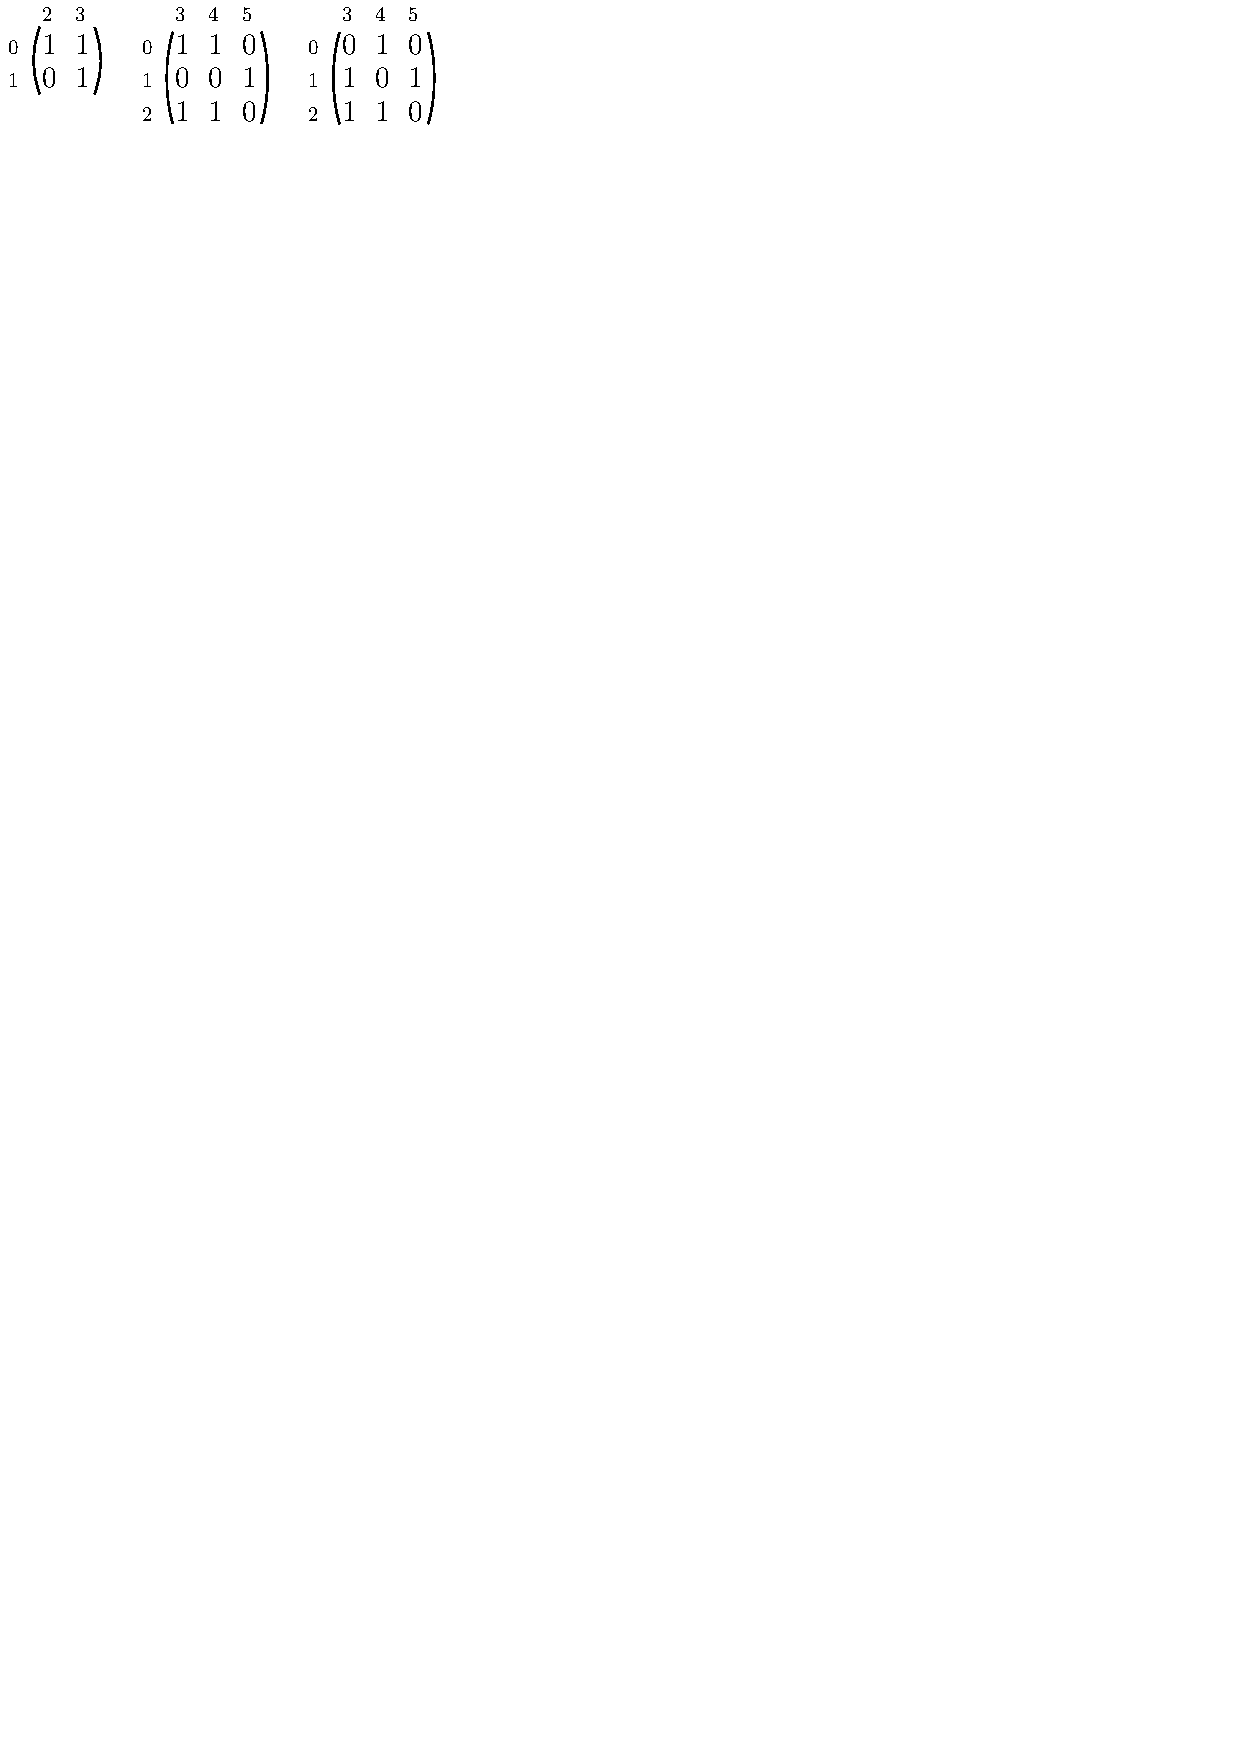
\includegraphics[width=100mm]{../img/avoiding.pdf}}}

Let the pattern $P$ be the left matrix from the picture. The middle matrix contains the pattern $P$, because a mapping $\{(0,0),(1,2),(2,3),(3,4)\}$ satisfies all the conditions. On the other hand the right matrix avoids the pattern as there is no such mapping.

There are other possible definitions of containing but from now on we will always consider a pattern to be contained as a submatrix. We will always denote $M$ the binary matrix for which we test the containing and by $P$ the pattern that is being tested. Moreover, we denote $h$ the height (the number of rows) of $P$ and $w$ its width.

\subsection*{Generating random matrix}
Our main goal is to show an iterated algorithm, which, with high enough number of iterations, for a given forbidden pattern and number $n$ generates a uniformly random binary matrix $M\in\{0,1\}^{n\times n}$ avoiding the pattern.

To create such an algorithm we generalize an algorithm generating fixed size permutations without a forbidden pattern introduced by [Madras-Liu]. To achieve randomness it uses Markov chain Monte Carlo method, which is explained in the next section.

The process starts with a binary matrix of the correct size avoiding the pattern (zero matrix is always sufficient) and in each step it changes uniformly at random one bit of the matrix and tests whether the matrix still avoids the pattern after the change. If it does the step is over, if it does not, we revert the change (flip the bit back) and end the step.

It can be proven that if the Markov chain is chosen carefully, this leads to a uniformly random matrix avoiding the pattern, after a sufficient number of steps. Sadly no-one knows what is ``sufficient'' in this manner of speaking.

\subsection*{Testing avoidance}
The hardest task to do in a step is to test whether the new matrix avoids the pattern. We show a very fast algorithm which only works for a special class of binary matrices as well as a slightly less performing algorithm for a general pattern, which again comes as a generalization of an algorithm for permutations from the article by Madras and Liu.
\addcontentsline{toc}{chapter}{Introduction}

